% Standard pen-and-paper worksheet preamble.
% Compile with: xelatex -interaction=nonstopmode exercise.tex   (run twice)
\documentclass[a4paper, 14pt]{extarticle}
\usepackage[top=1in, bottom=1in, left=1in, right=1in]{geometry}
\usepackage{amsmath}
\usepackage{amssymb}
\usepackage{graphicx}
\usepackage{hyperref}
\usepackage{tcolorbox}
\usepackage{enumitem}
\usepackage{multicol}
\usepackage{adjustbox}
\usepackage{etoolbox}
\usepackage{tikz}
\usepackage{fontspec}
\usetikzlibrary{calc,decorations,patterns,arrows,decorations.pathmorphing,positioning}
\definecolor{pltblue}{HTML}{1F77B4}

% Handwriting font. "Pretty Neat" (xkcd-style) is the house font; it is not
% installed everywhere, so guard it and fall back silently.
\newcommand{\ppfont}{}
\IfFontExistsTF{Pretty Neat}{
  \setmainfont{Pretty Neat}
  \renewcommand{\ppfont}{\fontspec{Pretty Neat}}
  \tikzset{every picture/.style={/utils/exec={\fontspec{Pretty Neat}}}}
  \AtBeginEnvironment{tabular}{\fontspec{Pretty Neat}}
}{
  \IfFontExistsTF{Humor Sans}{
    \setmainfont{Humor Sans}
    \renewcommand{\ppfont}{\fontspec{Humor Sans}}
    \tikzset{every picture/.style={/utils/exec={\fontspec{Humor Sans}}}}
    \AtBeginEnvironment{tabular}{\fontspec{Humor Sans}}
  }{}
}

% xkcd-style hand-drawn line decoration.
% WARNING: applying [xkcd] to many nodes can throw "Dimension too large".
% Use it on a handful of \draw lines only, never on every node.
\makeatletter
\pgfset{
  /pgf/decoration/randomness/.initial=2,
  /pgf/decoration/wavelength/.initial=100
}
\pgfdeclaredecoration{sketch}{init}{
  \state{init}[width=0pt,next state=draw,persistent precomputation={
    \pgfmathsetmacro\pgf@lib@dec@sketch@t0
  }]{}
  \state{draw}[width=\pgfdecorationsegmentlength,
  auto corner on length=\pgfdecorationsegmentlength,
  persistent precomputation={
    \pgfmathsetmacro\pgf@lib@dec@sketch@t{mod(\pgf@lib@dec@sketch@t+pow(\pgfkeysvalueof{/pgf/decoration/randomness},rand),\pgfkeysvalueof{/pgf/decoration/wavelength})}
  }]{
    \pgfmathparse{sin(2*\pgf@lib@dec@sketch@t*pi/\pgfkeysvalueof{/pgf/decoration/wavelength} r)}
    \pgfpathlineto{\pgfqpoint{\pgfdecorationsegmentlength}{\pgfmathresult\pgfdecorationsegmentamplitude}}
  }
  \state{final}{}
}
\tikzset{xkcd/.style={decorate,decoration={sketch,segment length=0.5pt,amplitude=0.5pt}}}
\makeatother

\setlength{\parindent}{0pt}
\setlength{\parskip}{0.5em}

\begin{document}

\section*{Do Your Friends Know Each Other?}

{\bf Question 1}:
Think of your two closest friends. Do those two know each other?
\underline{\hspace{2cm}}

Now suppose we pick two people at random out of everyone at this university.
Do \emph{they} know each other? \underline{\hspace{2cm}}

Your two friends were not picked at random --- they were picked by you. Write
down, in one sentence, why you think that changes the answer.

\underline{\hspace{\textwidth}}

\vspace{2em}

\section*{Part 1: Counting the closed corners}

Eight students share a dorm floor. Here is who eats lunch with whom.

\begin{center}
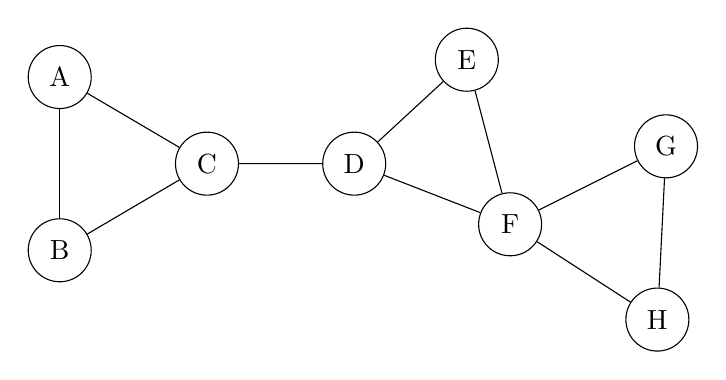
\begin{tikzpicture}[scale=1.1]
    \node[draw, circle, minimum size=8mm] (A) at (0,2.2) {A};
    \node[draw, circle, minimum size=8mm] (B) at (0,0.2) {B};
    \node[draw, circle, minimum size=8mm] (C) at (1.7,1.2) {C};
    \node[draw, circle, minimum size=8mm] (D) at (3.4,1.2) {D};
    \node[draw, circle, minimum size=8mm] (E) at (4.7,2.4) {E};
    \node[draw, circle, minimum size=8mm] (F) at (5.2,0.5) {F};
    \node[draw, circle, minimum size=8mm] (G) at (7.0,1.4) {G};
    \node[draw, circle, minimum size=8mm] (H) at (6.9,-0.6) {H};
    \draw (A) -- (B);
    \draw (A) -- (C);
    \draw (B) -- (C);
    \draw (C) -- (D);
    \draw (D) -- (E);
    \draw (D) -- (F);
    \draw (E) -- (F);
    \draw (F) -- (G);
    \draw (G) -- (H);
    \draw (H) -- (F);
\end{tikzpicture}
\end{center}

\begin{minipage}{\textwidth}
{\bf Question 2}:
Take one student at a time. List their lunch partners, count how many
\emph{pairs} of those partners could possibly eat together, and then count how
many of those pairs actually do. The row for A is filled in as an example.

\begin{center}
{\small
\begin{tabular}{|c|p{2.6cm}|c|p{2.2cm}|p{2.4cm}|p{1.8cm}|}
\hline
Student & Partners & How many & Pairs possible & Pairs connected & Fraction \\
\hline
A & B, C & 2 & 1 & 1 & 1 \\[0.35cm]
\hline
B & & & & & \\[0.45cm]
\hline
C & & & & & \\[0.45cm]
\hline
D & & & & & \\[0.45cm]
\hline
E & & & & & \\[0.45cm]
\hline
F & & & & & \\[0.45cm]
\hline
G & & & & & \\[0.45cm]
\hline
H & & & & & \\[0.45cm]
\hline
\end{tabular}
}
\end{center}
\end{minipage}

\clearpage

{\bf Question 3}:
The last column is called the \emph{local clustering coefficient} of a student.
Based on the numbers you just wrote:

\begin{enumerate}
    \item What does a value of 1 tell you about that student's social life?

    \underline{\hspace{\textwidth}}

    \item What would a value of 0 tell you?

    \underline{\hspace{\textwidth}}

    \item If a student has only one lunch partner, what should the value be ---
          and does your formula give an answer at all?

    \underline{\hspace{\textwidth}}
\end{enumerate}

{\bf Question 4}:
Average your eight fractions to get one number for the whole floor.

Average = \underline{\hspace{4cm}}

\vspace{2em}

{\bf Question 5}:
Now measure the same idea a completely different way, without looking at
individual students.

\begin{enumerate}
    \item Count the triangles on the floor --- groups of three students who all
          eat with each other. \underline{\hspace{2cm}}
    \item Count every ``corner'': a corner is a student together with two of
          their partners, whether or not those two eat together. (You already
          have this --- it is the ``pairs possible'' column, summed.)
          \underline{\hspace{2cm}}
    \item Every triangle gets counted as a closed corner three times, once at
          each of its three students. So the fraction of corners that are
          closed is

          \[
          \frac{3 \times (\text{triangles})}{\text{corners}} =
          \underline{\hspace{3cm}}
          \]
\end{enumerate}

{\bf Question 6}:
You now have two numbers that both claim to answer ``do friends of friends know
each other on this floor?'', and they disagree.

\begin{enumerate}
    \item Which one is larger? \underline{\hspace{2cm}}
    \item Student F has four partners and a low fraction. How many times does F
          count in the average of Question 4? \underline{\hspace{2cm}}
          How many corners does F contribute in Question 5?
          \underline{\hspace{2cm}}
    \item So which of the two measures listens more to the popular students,
          and which treats everyone equally?

    \underline{\hspace{\textwidth}}

    \item Two floors have identical numbers of triangles, but on one floor the
          triangles all sit around one very popular student. Which measure
          would notice the difference?

    \underline{\hspace{\textwidth}}
\end{enumerate}

\clearpage

\section*{Part 2: Compared to what?}

{\bf Question 7}:
Here are five students who \emph{all} eat with each other.

\begin{center}
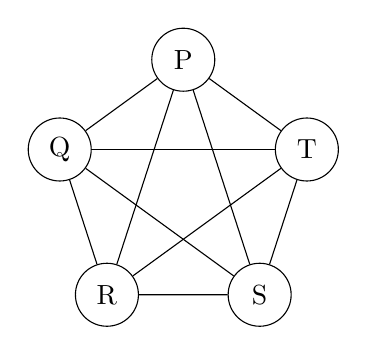
\begin{tikzpicture}[scale=1.1]
    \node[draw, circle, minimum size=8mm] (P) at (90:1.5) {P};
    \node[draw, circle, minimum size=8mm] (Q) at (162:1.5) {Q};
    \node[draw, circle, minimum size=8mm] (R) at (234:1.5) {R};
    \node[draw, circle, minimum size=8mm] (S) at (306:1.5) {S};
    \node[draw, circle, minimum size=8mm] (T) at (18:1.5) {T};
    \draw (P) -- (Q) -- (R) -- (S) -- (T) -- (P);
    \draw (P) -- (R); \draw (P) -- (S);
    \draw (Q) -- (S); \draw (Q) -- (T);
    \draw (R) -- (T);
\end{tikzpicture}
\end{center}

\begin{enumerate}
    \item Clustering of this group, by either recipe: \underline{\hspace{2cm}}
    \item Average number of handshakes between two of them:
          \underline{\hspace{2cm}}
    \item These are the best possible values: clustering as high as it goes,
          distance as short as it goes. Is this group a small world? Is it
          anything like a society?

    \underline{\hspace{\textwidth}}

    \item So a high clustering number and a low distance number, on their own,
          prove \underline{\hspace{5cm}}.
\end{enumerate}

\vspace{1em}

{\bf Question 8}:
To judge the dorm floor we need something to judge it \emph{against}. So build
a floor with no social structure at all: take the same 8 students, consider all
28 possible lunch pairs, and toss a biased coin for each one, keeping the pair
with probability $p$. Choose $p$ so that this coin-flip floor has, on average,
the same number of lunch pairs as the real one.

\begin{enumerate}
    \item How many lunch pairs does the real floor have?
          \underline{\hspace{2cm}} \quad So $p = $ \underline{\hspace{2cm}}
    \item On the coin-flip floor, take a student with 4 partners. Those partners
          form 6 possible pairs. Each of those 6 pairs is present with
          probability \underline{\hspace{2cm}}, so on average
          \underline{\hspace{2cm}} of them are present, and that student's
          fraction from Question 2 comes out to \underline{\hspace{2cm}}.
    \item Redo the previous item for a student with 2 partners, and one with 6.

    \underline{\hspace{\textwidth}}

    \item What is the clustering of a coin-flip floor, and what does it depend
          on? This is the punchline of Part 2 --- say it in one sentence.

    \underline{\hspace{\textwidth}}
\end{enumerate}

\clearpage

{\bf Question 9}:
Fill in the comparison. You already know how to compute distances by hand from
the first worksheet, so the two distance numbers are given to you here.

\begin{center}
\begin{tabular}{|l|p{3.2cm}|p{3.2cm}|}
\hline
 & Real dorm floor & Coin-flip floor \\
\hline
Clustering (average of Q2) & & \\[0.5cm]
\hline
Clustering (corner recipe, Q5) & & \\[0.5cm]
\hline
Average handshakes & 2.14 & 2.27 \\[0.5cm]
\hline
\end{tabular}
\end{center}

\begin{enumerate}
    \item How many times more clustered is the real floor than the coin-flip
          floor? \underline{\hspace{2cm}}
    \item How many times longer are its handshake chains?
          \underline{\hspace{2cm}}
    \item Combine your two answers into a single number that is large when a
          network is far more clustered than chance without paying for it in
          longer chains. Write your recipe.

    \underline{\hspace{\textwidth}}

    \item What value does your number take for the coin-flip floor itself?
          \underline{\hspace{2cm}} \quad What would it take for Ringville from
          the first worksheet --- bigger or smaller than that?
          \underline{\hspace{2cm}}
\end{enumerate}

{\bf Question 10}:
You used the average from Question 4. The student next to you used the corner
recipe from Question 5. Compute the number you invented in Question 9 both ways.

Yours: \underline{\hspace{3cm}} \quad Theirs: \underline{\hspace{3cm}}

You will both publish a paper claiming the dorm floor is a small world. What
must you report alongside the number for the claim to mean anything?

\underline{\hspace{\textwidth}}

\vspace{2em}

{\bf Question 11}:
Someone hands you a network you have never seen --- a power grid, a brain, a
citation network --- and asks: is it a small world? Write down the procedure
you would run. You do not have to compute anything; just list the steps in
order.

\vspace{8em}

\end{document}
